\documentclass[10pt,conference]{IEEEtran}

\usepackage{amsmath}
\usepackage{booktabs}
\usepackage{cite}
\usepackage{graphicx}
\usepackage{array}
\usepackage{pifont}
\usepackage{algorithm}
\usepackage{algpseudocode}
\usepackage{textcomp}
\usepackage{xcolor}
\usepackage{tikz}
\usepackage[hidelinks]{hyperref}
\usepackage{url}
\usetikzlibrary{positioning,arrows.meta}

\graphicspath{{figures/}}
\newcommand{\cmark}{\ding{51}}
\newcommand{\xmark}{\ding{55}}
\newcommand{\mr}{\mathrm{MR}}
\algtext*{EndIf}
\algtext*{EndFor}

\title{QMTester: Program-Level Metamorphic Testing for Quantum Programs}

\author{\IEEEauthorblockN{Anonymous Submission}}

\begin{document}

\bstctlcite{IEEEtranBSTCTL}

\maketitle

\begin{abstract}
A quantum program is more than its final \texttt{QuantumCircuit}: it is a builder, parameterized APIs, classical-register mappings, and ancilla protocols, and many real defects enter these program-level contracts before the circuit is emitted---invisible to a metamorphic transform that rewrites only the \emph{final} circuit. QMTester checks \emph{program-level} metamorphic relations over Qiskit by transforming a program input, rebuilding the circuit, and comparing canonicalized counts. Its discipline is \emph{canonicalization-as-admission}: a relation runs only when its output map is a documented bijection on the measured support, so a representation change is undone, not mistaken for a fault, and a register-dropping candidate rejected, not scored; admitted pairs go to a permutation two-sample test. Of five distribution-level families, two---qubit-role permutation and register remapping---and ancilla-uncompute defects crossing a non-unitary boundary need builder semantics: no MorphQ-class circuit transform diverges source from follow-up for a builder-ignores-input defect (\S\ref{sec:nonunitary}). The other two (QFT round-trip, parameter periodicity) are circuit-expressible, included for coverage; a complementary \emph{static} register-shape check covers the most common builder defect---the redundant \texttt{measure\_all} register the bijection excludes. Specificity is inclusion-independent: zero false positives over 107 fixed variants and 50 correct programs. Under realistic readout/crosstalk the smallest uncorrected $p$ narrows to $0.0035$, but the thin-margin subject's $m{=}96$ pairs give $\alpha/m{=}0.0005$, so the $0/50$ survive by correction, not luck, and real-defect detection holds $7/7$---though one cross-boundary \texttt{ancilla} variant, its family the most noise-sensitive, trips a false positive there. On ten real defects (seven Bugs4Q, three mined from recent Q\&A) it detects $10/10$ at $0$ false positives (Wilson $[0.722,1.000]$); on the seven it matches a reference-oracle ceiling with \emph{no} oracle, a \emph{deployable} static analyzer catches only the syntactic register-shape case, and MorphQ's $0/7$ is builder-layer blindness. An oracle-light ablation shows \emph{canonicalization}, not the statistic, carries detection---a minimal canonicalize-then-equality variant reaches $7/7$---while statistics carry specificity and the one probabilistic family (power floor at TVD$\approx0.02$--$0.03$). An exhaustive LintQ screen ($33{,}995$ findings) and an OOPSLA'22 corpus find distribution-detectable builder defects rare; the static check covers $37$ \texttt{measure\_all} findings. All numbers regenerate from frozen manifests and run-isolated shards.
\end{abstract}

\begin{IEEEkeywords}
quantum software testing, program-level metamorphic testing, builder-level relations, statistical testing, Qiskit
\end{IEEEkeywords}

\section{Introduction}

Quantum software is increasingly developed with familiar software-engineering workflows, but it is tested under an execution model that makes ordinary test oracles fragile. A quantum program usually returns samples from a distribution rather than a single deterministic value. The full quantum state is not directly observable without changing the computation, and the number of possible states grows exponentially with the number of qubits. Even when the intended circuit is correct, finite shots and backend noise can move observed frequencies enough to make exact-output assertions misleading. These properties turn regression testing into an oracle problem: developers need fault indicators without writing a fully specified expected distribution for every program and backend configuration~\cite{preskill2018quantum,huang2019statistical,li2020projection}.

A point that is easy to miss in this setting is \emph{where} the bug actually lives. A Qiskit program is not just the final \texttt{QuantumCircuit} object that reaches the backend. It is a builder that allocates qubits and classical registers, a set of parameterized APIs, a mapping from logical roles to wire indices, a measurement layout, and ancilla protocols that must uncompute cleanly. Many real defects are introduced at this program-contract layer---a permuted control qubit in a multi-controlled gate, a classical register read back in the wrong endianness, a QFT applied in the wrong direction, a rotation angle that breaks an intended periodicity, an ancilla that is never uncomputed---\emph{before} the concrete circuit is emitted. A metamorphic transformation that rewrites the \emph{final} circuit takes the buggy builder output as ground truth and rewrites around it; it therefore cannot expose a bug that is already baked into that output.

Existing work answers different parts of the oracle problem. Bugs4Q provides reproducible quantum-program defects for controlled studies~\cite{miao2023bugs4q}. MorphQ uses metamorphic transformations over generated circuits to expose faults in the Qiskit platform~\cite{paltenghi2023morphq}. Differential testing compares quantum software stacks when multiple implementations can run comparable programs~\cite{wang2021qdiff}. Assertion-based and projective-measurement approaches let developers encode stronger probabilistic or quantum-specific properties when those properties are known~\cite{huang2019statistical,li2020projection,oldfield2025faster}. These techniques operate at the \emph{circuit} or \emph{platform} level. We focus on the complementary boundary they leave open: the program/builder contracts that determine the circuit in the first place.

We target that boundary with QMTester, a metamorphic-testing workflow whose relations are defined over \emph{program inputs}, not over a fixed final circuit. Given a program subject---a builder plus the auditable semantics of its inputs---QMTester derives a follow-up \emph{input}, rebuilds the circuit from that follow-up input, executes the source and follow-up circuits under matched settings, canonicalizes the measured count vectors through a validated bijective map, and applies a corrected two-sample test to decide whether the program-level relation is violated. The relation families capture builder-level contracts: qubit-role covariance under input permutation, classical-register remapping, QFT round-trip direction, parameter periodicity, and ancilla uncompute. Each relation is admitted only under explicit, documented preconditions; a candidate that would change the number of measured bits, drop a register, or induce a non-bijective output map is rejected rather than tested.

We are deliberate about scope: we do not claim benchmark dominance over Bugs4Q, and the injected control is not evidence of real-world generality. Our calibrated, auditable claim is that on defects with a documented sound relation, program-level testing \emph{matches a ground-truth reference-oracle differential with no oracle}---not that it beats MorphQ, whose $0/7$ is structural blindness to the builder layer, not a comparative loss---at zero false positives on the matched fixed variants. A circuit-level-only diagnostic in our own artifact shows \emph{no} advantage over MorphQ, motivating the move to the program level rather than a larger circuit-level catalog.

The empirical account is traceable: every headline number resolves to a row of a canonical CSV derived from frozen manifests and run-isolated shards, and each included subject's relation-soundness audit is documented for inspection.

We make three contributions:
\begin{itemize}
  \item \textbf{A program-level instantiation of metamorphic testing for Qiskit.} We argue and demonstrate that a quantum program is a builder, parameterized APIs, register mappings, and ancilla protocols---not only its final circuit---and that defects in these contracts are a distinct target. For a \emph{builder-ignores-input} defect, no circuit-level metamorphic self-transform (the MorphQ class) can produce a source/follow-up divergence---it rewrites the already-emitted buggy circuit rather than re-invoking the builder on a different input---so detection requires rebuilding from a follow-up input (Proposition~1); this necessity holds structurally for qubit-role permutation and classical-register remapping, and across the non-unitary boundary (\S\ref{sec:nonunitary}) for ancilla-uncompute, whereas \texttt{program\_qft\_round\_trip} and \texttt{program\_parameter\_periodicity} are circuit-expressible and included for coverage.
  \item \textbf{Canonicalization-as-admission, in five distribution families plus a complementary static check.} The technical core is an admission discipline: a relation is tested only when its output map is a \emph{documented bijection on the measured support}, which separates a representation change from a logical divergence---candidates that drop a register or yield a non-bijective map are rejected, not scored. We instantiate it in five \texttt{program\_*} families (\texttt{input\_permutation}, \texttt{classical\_remap}, \texttt{qft\_round\_trip}, \texttt{parameter\_periodicity}, \texttt{ancilla\_uncompute}) under a quantum-aware period check (a $2\pi$ shift is rejected on a controlled rotation, whose period is $4\pi$), with a \emph{complementary static} \texttt{program\_register\_shape} check---needing no statistics---that brings the prevalent \texttt{measure\_all} register-shape defect in scope.
  \item \textbf{A prevalence finding (first-class), and an inclusion-independent evaluation.} An exhaustive screen of two real-defect corpora characterizes the niche precisely: distribution-detectable builder defects are \emph{rare}---the most common builder defect is the \texttt{measure\_all} register-shape change ($37$ of LintQ's $33{,}995$ findings), caught by the static register-shape check---so with all 32 build-and-run Bugs4Q bugs audited (9 in scope), we report a real-but-small niche rather than overstate it. Detection on the in-scope defects is \emph{deterministic} for all four real families (TVD~$=1$, the real QFT subject included) and holds $7/7$ under a realistic readout/crosstalk noise model; the statistics are load-bearing for specificity and the one probabilistic family, not for detection. The inclusion-\emph{independent} evidence is specificity (0/107 fixed variants, 0/50 correct programs; smallest per-pair $p=0.0035$ under the realistic model, Bonferroni still 0/50) and a detectability-unfiltered power curve (floor near TVD~$0.025$), plus an oracle-light ablation.
\end{itemize}

\section{Background and Related Work}

\subsection{Quantum Testing as an Oracle Problem}

Metamorphic testing replaces unavailable expected-output oracles with relations between executions of a program~\cite{chen1998metamorphic,barr2015oracle,segura2016survey,chen2018metamorphic}. Prior work reports that relation diversity can alleviate oracle weakness, while still depending on the quality of the chosen relations~\cite{liu2014effectively}. For quantum software, this idea is natural because many behavioral expectations are relational: equivalent circuits should induce the same measurement distribution, a logical qubit permutation should not change results after the output order is restored, and a global phase should not affect measurement probabilities. The difficulty is that these statements hold only under explicit preconditions.

The second difficulty is statistical. A source and follow-up execution can produce different empirical count vectors even when their true distributions are equal, while a real fault may produce a small distribution shift that is invisible under a low shot budget. Treating raw count equality as the oracle creates false alarms, while treating every p-value in isolation ignores the multiple follow-up executions generated per source program. We therefore combine relation validity with a corrected two-sample decision rule for categorical count data.

\subsection{Count Vectors and Output Canonicalization}
\label{sec:count-vectors}

A run of a quantum program produces a \emph{count vector}: a map from measured bitstrings to observed frequencies over $n$ shots. Comparing two runs is comparing two such vectors over a shared support. Two subtleties make this comparison non-trivial.

First, a valid relation often changes the \emph{representation} of the output without changing its logical content. Permuting input qubit roles, remapping a classical register, or reversing a QFT relabels which physical bit carries which logical value. Before any statistical test, QMTester rewrites the follow-up count vector into the source's logical order using a \emph{canonicalization} map $c$ induced by the transformation. A relation is admitted only when $c$ is a documented \emph{bijection} on the measured support: a candidate that drops a register, changes the number of measured bits, introduces a measurement where none existed, or yields a non-bijective map is rejected as a coverage loss, not scored as a test outcome.

Second, Qiskit exposes multi-register outputs as space-separated keys with register-dependent bit order and endianness. Canonicalization first flattens these keys and validates their length, then applies the relation's bijective remap. This is where representation bugs and genuine logical bugs are separated: if two logically equivalent program inputs disagree after a validated bijective remap, the disagreement is a candidate fault rather than a bookkeeping artifact.

\subsection{Non-Unitary Boundaries}
\label{sec:nonunitary}

Mid-circuit measurement, classical conditionals, reset, and other non-unitary operations break the simple ``rewrite-anywhere'' assumption that unitary metamorphic relations rely on. A transformation that is sound for a purely unitary prefix can be invalid once it crosses a measurement or a conditioned reset, because the operation's effect depends on a classical value produced at run time. Program-level relations must therefore declare, per family, whether and how they admit transformations across such boundaries. Several of our relations (e.g.\ ancilla uncompute and teleportation feedback) are specifically about getting these boundaries right, which is why they are expressed over the program's builder semantics rather than over the emitted circuit.

\subsection{Positioning}

We position QMTester by oracle assumption, evidence model, and \emph{testing level} in Table~\ref{tab:related-comparison}. MorphQ is the closest baseline because it also uses metamorphic testing in the Qiskit ecosystem. The decisive distinction is the level at which relations are defined: MorphQ is a \emph{circuit-level} baseline that transforms a generated or given final circuit, whereas QMTester defines relations over \emph{program inputs} and rebuilds the circuit from the follow-up input. This is not a statement that MorphQ is weak. It means MorphQ structurally cannot exploit builder-level semantics: when a defect is already present in the final circuit a builder produced, a circuit-level transformation rewrites a faithful copy of the buggy output and observes no inconsistency. A MorphQ score of $0/7$ on our audited program-level subset is therefore an inherent consequence of the testing level, not an unfair comparison or a tuning artifact.

\begin{table*}[t]
\centering
\caption{Positioning against related quantum testing work. The decisive axis is the \textbf{testing level}: QMTester defines relations over \emph{program/builder inputs}, whereas MorphQ and related metamorphic tools transform a \emph{final circuit}.}
\label{tab:related-comparison}
\scriptsize
\setlength{\tabcolsep}{2.5pt}
\begin{tabular}{@{}p{0.12\textwidth}p{0.10\textwidth}p{0.17\textwidth}p{0.18\textwidth}p{0.30\textwidth}@{}}
\toprule
\textbf{Work} & \textbf{Testing level} & \textbf{Primary focus} & \textbf{Oracle / evidence model} & \textbf{Relationship to QMTester} \\
\midrule
\textbf{QMTester (ours)} & Program / builder & Metamorphic testing of Qiskit program inputs & Program-relation violation via canonicalized count-vector test & --- \\
MorphQ~\cite{paltenghi2023morphq} & Circuit / platform & Metamorphic testing of the Qiskit platform & Generated final-circuit pairs and platform-level failures & Closest baseline; circuit-level, so it cannot reach builder-layer contracts (hence $0$ on the audited program-level subset). \\
Bugs4Q~\cite{miao2023bugs4q} & --- (benchmark) & Reproducible quantum-program bugs & Curated bug/fix pairs & Real-defect substrate; we use an audited program-level subset with documented relations. \\
QDiff~\cite{wang2021qdiff} & Stack & Differential testing across stacks & Cross-stack output discrepancies & Complementary; needs comparable implementations across stacks. \\
QMutPy~\cite{fortunato2022qmutpy} & Circuit / suite & Mutation testing for Qiskit & Existing tests kill or survive mutants & Related only; \emph{not evaluated} here---assumes a test suite, not an oracle-light baseline. \\
QOPS/SB-QOPS~\cite{muqeet2024qops,muqeet2026sbqops} & Circuit & Pauli-string and search-based testing & Measurement-centric Pauli-string oracles & Strong oracle-centered alternative; targets settings with Pauli specifications. \\
QEMI~\cite{luo2026qemi} & Stack & EMI-style stack testing & Dead-code variants should preserve behavior & Complementary metamorphic direction over dead-code variants. \\
Statistical assertions~\cite{huang2019statistical} & Program & Probabilistic program assertions & Developer-specified probability properties & Statistical discipline but requires absolute probability specifications. \\
Projective-measurement testing~\cite{li2020projection,oldfield2025faster} & Circuit & Efficient assertion checking & Projective predicates and reduced measurements & Complementary route to stronger or cheaper relation-specific oracles. \\
\bottomrule
\end{tabular}
\end{table*}


Closest to our setting is the quantum metamorphic-testing line itself. Abreu et al.~\cite{abreu2022metamorphic} and Costa et al.~\cite{costa2022asserting} develop metamorphic relations for oracle and Shor-style quantum programs, while MorphQ~\cite{paltenghi2023morphq} and its reproducibility follow-up MorphQ++~\cite{kitt2024morphqpp} apply metamorphic transformations to the Qiskit quantum platform. These works define relations primarily over the \emph{circuit} (or over an algorithm-level specification) and transform an already-emitted circuit. QMTester differs on two axes that matter for builder-layer defects: (i) its relations are defined over \emph{program/builder inputs} and the follow-up circuit is \emph{rebuilt} from the transformed input rather than rewritten from the source circuit, and (ii) a candidate is admitted only when its output canonicalization is a validated bijection on the measured support. The first axis is what lets a relation see a defect the buggy builder bakes into its circuit; the second is what prevents a representation change from being scored as a fault. We retain MorphQ as the matched circuit-level baseline because it is the most directly runnable tool on the same Qiskit subjects; the contrast with these algorithm/circuit-level relations is about the testing \emph{level}, not tool quality.

The comparison also clarifies what we do not claim. We do not replace proof-oriented formal methods for programs with available specifications, and we do not make Pauli-string or projective assertions unnecessary when such specifications are known. Quantum Hoare logics, relational logics, embedded circuit languages, and circuit-equivalence checkers offer stronger reasoning obligations when their models and specifications apply~\cite{ying2011hoare,unruh2019qrhl,paykin2017qwire,peham2022zx}. We use those ideas as a boundary: QMTester checks empirically whether admitted source/follow-up program pairs behave consistently, but it is not a platform differential-testing campaign, a mutation-adequacy metric, a proof system, or a device-backed study. We also do not evaluate QMutPy in this submission; mutation testing assumes an existing test suite and is not a substitute for the oracle-light, builder-level use case we target.

\section{QMTester Approach}

We design QMTester as a paired-execution workflow over \emph{program inputs}. The input is not a fixed circuit but a \emph{program subject}: a Qiskit builder together with the auditable semantics of its inputs (qubit roles, classical-register layout, parameters, ancilla protocol), a backend configuration, a shot budget, and a set of enabled program-level relation families. The output is a set of relation-level decisions plus a source-level detection decision after multiple-testing correction. Figure~\ref{fig:architecture} summarizes the workflow.

\begin{figure}[t]
\centering
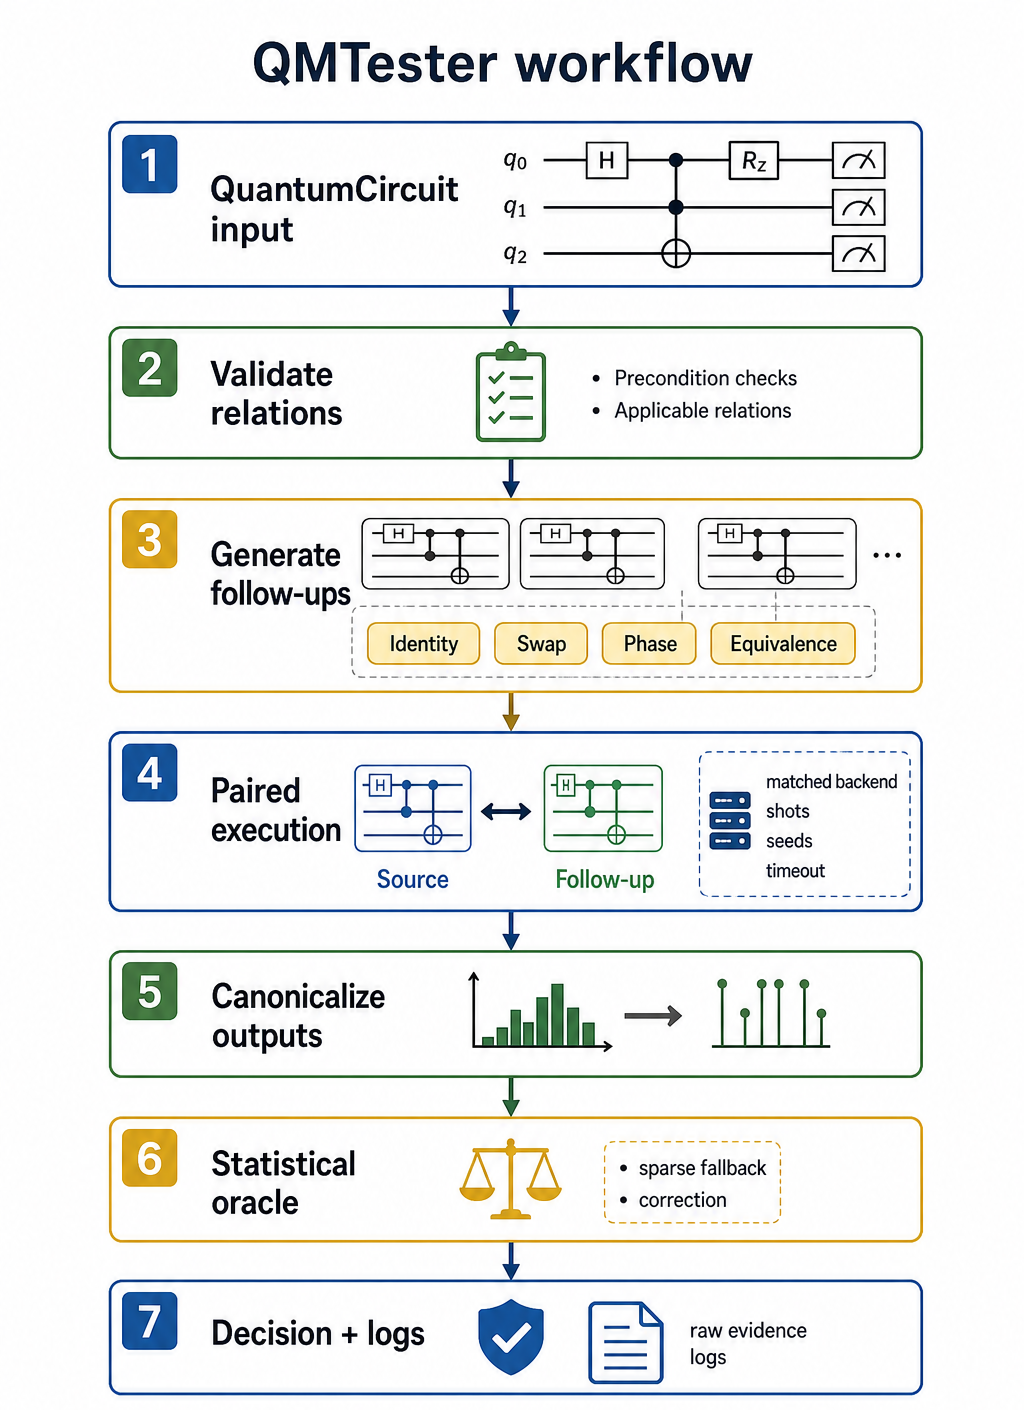
\includegraphics[width=\columnwidth]{architecture_ai.png}
\caption{QMTester workflow: a program subject yields source and follow-up \emph{inputs}; the builder produces source and follow-up circuits; paired execution yields count vectors; canonicalization validates and remaps outputs; a statistical oracle flags relation violations.}
\label{fig:architecture}
\end{figure}

\subsection{Two-Layer Design}

QMTester is organized as two layers with a clean interface between them.

\noindent\textbf{Layer 1: relation admission and canonicalization.} This layer is subject-agnostic. It admits a candidate transformation only under its declared preconditions, builds the source and follow-up circuits, executes them under matched settings, and canonicalizes the resulting count vectors through a validated bijective map before any test is run (Sec.~\ref{sec:count-vectors}). A candidate whose canonicalization map is not bijective on the measured support, or that changes the measured-bit count, drops a register, or crosses a non-unitary boundary a family does not admit, is rejected and logged as a coverage loss rather than scored.

\noindent\textbf{Layer 2: program-level subject adapters and relation families.} This layer encodes the auditable builder-level semantics of each subject. A \texttt{ProgramSubject} adapter exposes how to construct the circuit from a given input and what each input position means (which qubit plays which role, which classical bit records which logical value, which parameter must respect which periodicity, which register is an ancilla). A \texttt{ProgramRelationCandidate} pairs a subject with a relation family and produces the follow-up \emph{input} together with the induced canonicalization map. Because the relation is expressed over inputs and the circuit is \emph{rebuilt} from the follow-up input, a defect that a buggy builder bakes into its output is exposed as a divergence between the source and follow-up outputs.

\subsection{Workflow}

We split the workflow into five stages (Fig.~\ref{fig:architecture}'s boxes further split stage one into input/validate and stage five into canonicalize/oracle/decision). Stage one normalizes the source subject metadata so that qubit roles, classical registers, measurement layout, and output-bit order are explicit. Stage two enumerates candidate follow-up inputs from the enabled relation families. Stage three checks each candidate against its relation-specific preconditions and constructs the induced canonicalization map before admitting a follow-up. Stage four rebuilds and executes the source and follow-up circuits under the same backend, shot budget, seed policy, and timeout policy. Stage five canonicalizes the observed count vectors and compares them with the statistical oracle.

\begin{algorithm}[t]
\caption{QMTester program-level detection pipeline}
\label{alg:qmtester}
\scriptsize
\begin{algorithmic}[1]
\Require subjects $\mathcal{S}$, program relations $\mathcal{R}$, backend $b$, shots $n$, seeds, timeout $\tau$, threshold $\alpha$
\Ensure pair logs, source decisions, rejected relation records
\ForAll{$P \in \mathcal{S}$}
  \State $Pairs \gets [\,]$; $Rejects \gets [\,]$
  \ForAll{$R \in \mathcal{R}$}
    \ForAll{$\iota' \in \Call{FollowUpInputs}{R,P}$}
      \If{$\Call{Admissible}{P,R,\iota'}$}
        \State $c \gets \Call{CanonMap}{P,R,\iota'}$
        \State $Pairs \gets Pairs \cup \{(R,P,\Call{Build}{P,\iota'},c)\}$
      \Else
        \State $Rejects \gets Rejects \cup \{(P,R,\iota',\Call{Reason}{P,R,\iota'})\}$
      \EndIf
    \EndFor
  \EndFor
  \State $Tests \gets [\,]$
  \ForAll{$(R,P,P',c) \in Pairs$}
    \State $x \gets \Call{Execute}{P,b,n,seeds,\tau}$
    \State $y \gets \Call{Execute}{P',b,n,seeds,\tau}$
    \State $(x,y) \gets \Call{Canonicalize}{x,y,c}$
    \State $(p,sparse) \gets \Call{TwoSampleTest}{x,y}$
    \If{$sparse$}
      \State $p \gets \Call{ExactOrResample}{x,y}$
    \EndIf
    \State $Tests \gets Tests \cup \{(R,p,sparse)\}$
  \EndFor
  \State $\alpha_{\mathrm{eff}} \gets \alpha/|Tests|$
  \State $detected \gets \exists(R,p,s) \in Tests: p < \alpha_{\mathrm{eff}}$
  \State \Call{WriteLogs}{$P,Pairs,Tests,Rejects$}
  \State \Call{WriteDecision}{$P,detected,\alpha_{\mathrm{eff}}$}
\EndFor
\end{algorithmic}
\end{algorithm}

We make the procedure intentionally conservative about invalid relations. A follow-up input that cannot be justified under the subject's role semantics, parameter domain, classical-control behavior, or canonicalization bijectivity is rejected before execution. This rejection reduces relation coverage, but it prevents QMTester from treating a self-inflicted semantic change as a program fault.

\subsection{Formal Model and Assumptions}

We use the formal model to mark exactly where QMTester relies on relation validity and where it relies on statistical testing. Let $P$ be a program subject with input $\iota$ that builds a circuit $\mathrm{Build}(P,\iota)$ whose measurement outcomes range over bitstrings $B(P)$. A program relation family $R$ induces candidate follow-up inputs $\iota'$; the predicate $A_R(P,\iota')$ records whether the relation's preconditions are satisfied and whether the induced map $c_R:B(\mathrm{Build}(P,\iota'))\rightarrow B(\mathrm{Build}(P,\iota))$ is bijective on the measured support. If $A_R(P,\iota')$ holds, QMTester admits the follow-up circuit $P'=\mathrm{Build}(P,\iota')$ and records $c_R$. Under a fixed execution setting $e$, repeated executions yield empirical count vectors $\hat{D}_{P,e}$ and $\hat{D}_{P',e}$ that estimate the corresponding measurement distributions defined by the circuit semantics and Born rule~\cite{nielsen2010quantum}.

We deliberately separate relation obligations from statistical decisions. When the admitted relation is valid for $P$ and the builder implements the intended semantics, then $D_{P,e}(b)=D_{P',e}(c_R^{-1}(b))$ for every observable bitstring $b$ after canonicalization. This is a conditional obligation, not an implementation-level proof; the artifact exposes admitted and rejected follow-up inputs so readers can audit $A_R$ on concrete subjects. For each admitted pair, QMTester tests $H_0:D_{P,e}=c_R(D_{P',e})$ against a distributional alternative.

\noindent\textbf{Remark 1 (source-level Bonferroni control).} For one source subject with $m$ admitted follow-up pairs, rejecting when any pair has $p_i<\alpha/m$ controls the source-level false-alarm probability at $\alpha$ when all $m$ nulls hold: each valid null has $\Pr[p_i<\alpha/m]\leq\alpha/m$, and the union bound gives $\Pr[\exists i:p_i<\alpha/m]\leq\alpha$. This is the standard Bonferroni bound; its only non-trivial content is the premise that the per-pair nulls are \emph{valid}, which is exactly what the empirical type-I check of Sec.~\ref{sec:oracle-behavior} probes (and finds conservative rather than uniform). The bound covers neither invalid relations nor unaudited raw logs.

\subsection{Fault Model and Scope}
\label{sec:fault-model}

We target faults that manifest as changes in the measured output distribution under a transformation of program inputs that should preserve observable behavior. Examples include permuted qubit roles in multi-controlled gates, wrong classical-bit indexing or endianness, inverted QFT direction, parameter values that break an intended periodicity, and ancillas that are not uncomputed. Such faults are common in quantum-program benchmarks because small builder-level mistakes can leave code type-correct while changing the program's observable behavior.

We do not claim coverage of all quantum bugs. A fault that preserves the measured distribution for the selected input and relation family will not be detected. A fault whose effect size is smaller than the available shot budget may also evade the statistical oracle. Faults that require semantic knowledge outside the program, such as an application-specific cost-function expectation, may need assertions or domain-specific relations. These boundaries define the method's scope rather than exceptions discovered after evaluation.

\subsection{Program-Level Metamorphic Relations}
\label{sec:relations}

We organize follow-up generation into five program-level relation families, each defined over program inputs and each carrying a documented soundness argument and a bijective canonicalization map.

\begin{itemize}
  \item \texttt{program\_input\_permutation}: permute the logical roles of input qubits in a way the subject's semantics declare covariant, and restore the output order by the inverse permutation. Detection does \emph{not} rest on symmetric-control invariance (which a correct builder satisfies trivially): in our \texttt{ccx\_role} subject the buggy builder hard-codes \texttt{ccx(0,1,2)} (target on wire~2) and ignores the requested role map, so permuting the input roles moves the state-prep gates but not the hard-coded \texttt{ccx}, and the canonicalized source/follow-up diverge; the role-covariant fix (\texttt{ccx(2,1,0)}) moves the gate too and stays equal, raising no false positive.
  \item \texttt{program\_classical\_remap}: remap the classical-register layout (order/endianness) under which results are recorded, then canonicalize back to the source layout. Targets measurement-order and endianness contracts.
  \item \texttt{program\_qft\_round\_trip}: compose the program's QFT stage with its declared inverse so the round trip is the identity on the logical input. Targets QFT-direction and rotation-sign defects.
  \item \texttt{program\_parameter\_periodicity}: shift a rotation parameter by a full intended period so the observable distribution is unchanged. The admission check is period-aware: a $2\pi$ shift is sound for an uncontrolled Pauli rotation (the extra $-1$ is a global phase) but a \emph{controlled} Pauli rotation has period $4\pi$ (the $-1$ becomes relative), so a $2\pi$ declaration on a controlled rotation is rejected as an invalid context rather than tested---a confusion documented in production Qiskit~\cite{qiskit13670}.
  \item \texttt{program\_ancilla\_uncompute}: require that ancilla and feedback registers return to a clean state, so adding or completing the declared uncompute leaves the logical output invariant. Targets missing/incorrect uncompute, teleportation feedback, and Grover ancilla protocols.
  \item \texttt{program\_register\_shape}: a \emph{complementary static check}, not a distribution relation---a builder asked to report in its declared $n$-bit register must emit that shape, which the prevalent \texttt{measure\_all} defect violates by doubling the output to $2n$ bits. Needing no statistics, it is the one case a deployable static analyzer also reaches (Table~\ref{tab:program-baselines}); it brings \texttt{qiskit\_github\_12} and the 37 LintQ \texttt{measure\_all} findings (\S\ref{sec:threats}) in scope.
\end{itemize}

\begin{table*}[t]
\centering
\caption{Program-level relation-validity obligations for QMTester. Each relation is defined over \emph{program inputs}; the follow-up circuit is rebuilt from the follow-up input and its outputs are remapped through a validated bijective canonicalization map before testing.}
\label{tab:relation-validity}
\scriptsize
\setlength{\tabcolsep}{2.2pt}
\begin{tabular}{@{}p{0.15\textwidth}p{0.17\textwidth}p{0.14\textwidth}p{0.15\textwidth}p{0.16\textwidth}p{0.13\textwidth}@{}}
\toprule
\textbf{Relation family} & \textbf{Preconditions} & \textbf{Invariant} & \textbf{Target bug classes} & \textbf{Invalid contexts} & \textbf{Implementation checks} \\
\midrule
\texttt{program\_input\_permutation} & Subject declares a covariant permutation of input qubit roles (e.g.\ symmetric controls); inverse permutation restores output order. & Canonicalized bitstring distribution matches the source after the inverse role permutation. & Qubit-role bookkeeping in multi-controlled and symmetric constructions. & Permutations the subject does not declare covariant; untracked classical side effects. & Validate role permutation, bijective inverse, and classical-bit remapping. \\
\texttt{program\_classical\_remap} & Classical-register layout (order/endianness) is remappable and canonically invertible to the source layout. & Logical outcome distribution is invariant after remapping classical bits to source order. & Measurement-order and endianness contracts. & Remaps that drop or duplicate classical bits, or change the measured-bit count. & Validate bijective register map, key length, and flatten/endianness handling. \\
\texttt{program\_qft\_round\_trip} & Subject exposes a QFT stage with a declared inverse over the same ordered qubits. & QFT composed with its inverse acts as the identity on the logical input. & QFT-direction and rotation-sign defects. & Approximate or truncated QFT without a matching inverse; mismatched qubit order. & Check QFT/inverse pairing, qubit order, and round-trip identity. \\
\texttt{program\_parameter\_periodicity} & Rotation parameter has a declared period $T$; shifting by $T$ preserves the observable. & Measurement distribution is invariant under a full-period parameter shift. & Angle handling and periodicity contracts (also drives hard mutants). & Parameters whose period is not declared or is broken by the subject; non-periodic gates. & Confirm declared period and reject shifts outside the periodic domain. \\
\texttt{program\_ancilla\_uncompute} & Ancilla/feedback registers are declared and must return to a clean state. & Completing the declared uncompute leaves the logical output invariant. & Missing/incorrect uncompute, teleportation feedback, Grover ancilla protocols. & Transformations that leave an ancilla entangled or cross a non-unitary boundary the family does not admit. & Verify ancilla cleanliness, feedback handling, and uncompute completion. \\
\bottomrule
\end{tabular}
\end{table*}


Our design goal is distinct builder-level contracts, not a universal relation. We distinguish families by \emph{why} circuit-level testing misses them. \texttt{program\_input\_permutation}, \texttt{program\_classical\_remap}, and largely \texttt{program\_ancilla\_uncompute} are \emph{structurally} builder-only: no circuit-level metamorphic \emph{self}-transform recovers the qubit-role mapping, register layout/endianness, or ancilla identity, because it rewrites the emitted circuit rather than rebuilding from a different input. By contrast \texttt{program\_parameter\_periodicity}, and \texttt{program\_qft\_round\_trip} where the QFT block is identifiable, are \emph{circuit-expressible}: a period shift is a local gate edit a circuit-level tool could in principle apply, so MorphQ's $0$ there reflects a \emph{catalog gap}, not structural invisibility---the necessity claim holds strictly for the structurally builder-only families, which Proposition~1 formalizes. (The one mined QPE subject is \emph{incidentally} flagged by a circuit-level swap rewrite---perturbing its wiring, not recovering the role map---so the structural argument is intact.)

\noindent\textbf{Proposition~1 (Necessity for builder-ignores-input defects).}
\label{prop:necessity}
Let a \emph{self-transform} be any MorphQ-class circuit transform---identity insertion, equivalence-preserving relabeling, phase or equivalence rewriting---that rewrites the emitted circuit $C=\mathrm{Build}(P,\iota)$ into a $C'$ preserving its unitary, hence its distribution ($D_{C'}=D_C$). For a \emph{builder-ignores-input} defect (e.g.\ \texttt{ccx\_role}), where the buggy builder hard-codes gates independently of $\iota$, no self-transform yields a source/follow-up divergence: it never re-invokes the builder, so the pair agrees by construction. Exposing the defect requires \emph{rebuilding} from a different input $\iota'$---the input-level relation $A_R$. For ancilla-uncompute the obstruction is the same, the missing uncompute crossing the non-unitary boundary (\S\ref{sec:nonunitary}) an equivalence-preserving rewrite may not cross. This is \emph{not} the false claim that information is lost on emission: a reference-oracle differential recovers all seven (Table~\ref{tab:program-baselines}) by comparing $C$ against a \emph{different} correct circuit---what no self-transform synthesizes from $C$ alone, but rebuilding from $\iota'$ supplies oracle-free. Table~\ref{tab:relation-validity} is part of the method: each row implies negative tests for the generator (e.g.\ \texttt{program\_classical\_remap} must reject non-bijective maps). A purely circuit-level catalog is retained only as a diagnostic baseline (\S\ref{sec:diagnostic}), where it shows no advantage over MorphQ.

\subsection{Statistical Oracle}
\label{sec:statistical-oracle}

After output canonicalization, we treat observed shot counts from $P$ and admitted follow-up $P'$ as samples from categorical distributions $D_P$ and $D_{P'}$ over the aligned support $B(P)$, testing $H_0: D_P = D_{P'}$ against the alternative that the distributions differ. \emph{The oracle is a Monte-Carlo permutation two-sample test}: we draw $B=10{,}000$ relabelings of the pooled shots and read the p-value off the permutation reference (\S\ref{sec:oracle-behavior}; sparse-cell mechanics below). An asymptotic $\chi^2$ fast path exists for dense supports but is not the operative branch on our exponentially sparse quantum outputs (zero cell-merges across all admitted pairs; the permutation branch decides $\geq 85.7\%$ of pairs), so it is reported, not relied on. The permutation statistic is the pooled-denominator two-sample form
\[
\begin{gathered}
T = \sum_{k=1}^{K} \frac{(x_k - e_k)^2 + (y_k - f_k)^2}{e_k + f_k},\\[2pt]
e_k=\tfrac{n_x(x_k+y_k)}{n_x+n_y},\quad f_k=\tfrac{n_y(x_k+y_k)}{n_x+n_y},
\end{gathered}
\]
for source/follow-up shot totals $n_x, n_y$. $T$ is a monotone transform of the standard Pearson two-sample statistic~\cite{pearson1900criterion}---one-half of it under matched totals $n_x=n_y$---so the permutation reference, which decides the vast majority of pairs, is unaffected by the choice. (The $\chi^2_{K'-1}$ fast path acts on the \emph{standard} Pearson statistic; per above it is untaken here.)

\noindent\textbf{Sparse-cell handling.}
Quantum outputs are sparse because the support $\{0,1\}^q$ grows exponentially with the qubit count $q$. The chi-squared approximation degrades when too many cells have small expected counts. We use a two-stage rule with explicit thresholds rather than a single heuristic:
\begin{enumerate}
  \item \emph{Cell merging.} Sort cells by $e_k$ ascending. Merge any cell with $e_k<5$ into a single ``other'' bin (Cochran's rule). If after merging the number of effective bins $K'$ satisfies $K'\geq 5$ \emph{and} at least 80\% of bins have $e_k\geq 5$, we accept the asymptotic chi-squared p-value.
  \item \emph{Exact / resampling fallback.} Otherwise we mark the pair \texttt{sparse=true} and use a Monte-Carlo permutation test on the pooled multinomial: we draw $B=10{,}000$ permutations of the $n_x+n_y$ pooled shots into two groups of size $n_x$ and $n_y$, recompute $\chi^2$, and report $\hat{p} = (1+\#\{b: \chi^2_b \geq \chi^2_{\mathrm{obs}}\})/(B+1)$. The branch is logged per pair so readers can recompute either from raw counts.
\end{enumerate}
As noted above, the fast path is not the operative branch on our corpus (zero cell-merges; $K'=K$ throughout), and the permutation branch decides $\geq 85.7\%$ of pairs (\S\ref{sec:oracle-behavior}).

\noindent\textbf{Multiple-testing correction.}
QMTester applies Bonferroni correction over all admitted follow-up pairs generated for the same source subject. With $m$ pairs and family-wise threshold $\alpha=0.05$, the default per-pair threshold is $\alpha/m$; step-down Holm correction is reported as a sensitivity check but is not mixed with the default decision rule~\cite{holm1979simple}. We use the source subject rather than the whole benchmark as the correction unit. This choice controls the chance that one subject is flagged because many follow-up variants were tried, while avoiding an overly conservative threshold that couples unrelated subjects.

\noindent\textbf{Noisy-simulator calibration.}
On noisy backends, two executions of the \emph{same} source circuit under independent seeds can produce statistically distinguishable count vectors purely from backend variability. We separate that variability from a real follow-up deviation by executing $P$ under $K=20$ independent seeds at shot budget $n$, computing the $\binom{K}{2}=190$ pairwise null statistics after the same canonicalization and sparse-cell rule, and using the $(1-\alpha/m)$-quantile as the calibrated rejection threshold $\hat\tau_P$ for that subject. The calibration runs are logged separately so readers can recompute $\hat\tau_P$ from the 20 raw count vectors. This procedure is a pragmatic complement to learned noise-mitigation methods~\cite{muqeet2024noise} and does not require a noise model.

We report all detection and false-positive rates with Wilson 95\% confidence intervals~\cite{wilson1927probable}, and the artifact records, for every admitted pair, the raw count vectors, $\chi^2$ statistic, asymptotic p-value, sparse-cell decision, fallback p-value (if applicable), and Bonferroni-corrected threshold. The prototype is a Python workflow over Qiskit's \texttt{QuantumCircuit}; all reported claims are simulator-based, and device evaluation is out of scope (Sec.~\ref{sec:threats}).

\section{Evaluation}

We organize the evaluation around four program-level research questions---RQ1 (audited Bugs4Q defects), RQ2 (balanced injected positive control), RQ3 (false positives), and RQ4 (sensitivity floor)---plus a circuit-level-only diagnostic run (\S\ref{sec:diagnostic}). Each claim is tied to a dataset, baseline, and metric, and each dataset is introduced with its research question below. MorphQ is the only matched baseline; QMutPy is not evaluated (it assumes an existing test suite), and stack/assertion tools are related-only comparators (Table~\ref{tab:related-comparison}). The primary evidence is program-level; the circuit-level run is retained only as a diagnostic and is not used as a main claim.

\subsection{Execution and Evidence Pipeline}

All runs use Qiskit Aer under a pinned environment, a fixed master seed, a default shot budget for detection, and a per-pair wall-clock timeout. MorphQ is run on the same subjects under identical backends, shot budgets, seeds, and timeouts. Every headline number resolves to one row of a canonical CSV that is derived by \texttt{derive\_metrics.py} from run-isolated summary shards under a frozen run directory; the derivation enforces expected denominators, rejects missing or stale-mixed rows, and re-derives the canonical CSV to a byte-identical copy (\emph{canonical integrity check: PASS}). Table~\ref{tab:canonical-results} is the canonical view.

\begin{table*}[t]
\centering
\caption{Canonical results, regenerated from the frozen run's \texttt{canonical\_results.csv}. Intervals are Wilson 95\% CIs. MorphQ's program-level detections are $0$ by the testing level (Sec.~\ref{sec:relations}). $^{\dagger}$Coverage-by-construction (admit-if-detected), not a detection rate (Sec.~\ref{sec:threats}). $^{\S}$The 3 mined subjects (\S\ref{sec:rq1}) meet the same checks but lie outside the frozen run. $^{\flat}$Degenerate cell (matched seeds give $p\equiv1$); the noisy/calibrated rows are informative.}
\label{tab:canonical-results}
\scriptsize
\setlength{\tabcolsep}{2.4pt}
\begin{tabular}{@{}p{0.16\textwidth}p{0.20\textwidth}p{0.12\textwidth}p{0.13\textwidth}p{0.08\textwidth}p{0.16\textwidth}@{}}
\toprule
\textbf{Cohort} & \textbf{Benchmark} & \textbf{Method} & \textbf{Metric} & \textbf{Count} & \textbf{Rate [95\% CI]} \\
\midrule
Audited Bugs4Q & Program-level defect subset & QMTester & Detected & 7/7 & 1.000 [0.646, 1.000] \\
Real defects (all)$^{\S}$ & Bugs4Q $+$ 3 mined (QCSE) & QMTester & Detected & \textbf{10/10} & \textbf{1.000 [0.722, 1.000]} \\
Audited Bugs4Q & Program-level defect subset & MorphQ & Detected & 0/7 & 0.000 [0.000, 0.354] \\
Program injected$^{\dagger}$ & 100-case positive-control & QMTester & Detected & 100/100 & coverage-by-constr. \\
Program injected & 100-case positive-control & MorphQ & Detected & 20/100 & 0.200 [0.133, 0.289] \\
Fixed variants & 7 Bugs4Q + 100 injected fixed & QMTester & False pos. & 0/107 & 0.000 [0.000, 0.035] \\
Correct programs$^{\flat}$ & ideal / noisy / calibrated sim & QMTester & False pos. & 0/50 \emph{each} & 0.000 [0.000, 0.071] \\
\bottomrule
\end{tabular}
\end{table*}


\subsection{RQ1: Real Program-Level Defects}
\label{sec:rq1}

\noindent\textbf{How many audited Bugs4Q program-level defects does QMTester detect?}

We \emph{included} a Bugs4Q subject only when a sound program-level relation could be justified (an input transform, a bijective canonicalization map, and a soundness argument tied to builder semantics). The denominators form one \emph{closed} chain: of the 42 Bugs4Q bugs~\cite{miao2023bugs4q}, 32 build and run under our pinned Qiskit (the diagnostic set, \S\ref{sec:diagnostic}); we audited \emph{all 32} (per-bug dispositions in the artifact), of which \emph{9} admit a sound builder-contract relation and 23 are out of scope (12 api-misuse, the rest output-formatting, platform/runtime, or wrong-gate; Table~\ref{tab:excluded-bugs4q}). Seven of the nine are runnable distribution-family subjects (Table~\ref{tab:audited-bugs4q}), all detected; the \texttt{program\_register\_shape} static check flags the eighth---\texttt{qiskit\_github\_12}, the \texttt{measure\_all} defect previously excluded for lacking a bijective map---and the ninth (a QPE/inverse-QFT case) awaits a sound relation. QMTester thus \emph{handles 8} of the 9 admitted defects (7/7 on the distribution families) and flags none of the matched fixed variants. Beyond Bugs4Q, mining recent Quantum Computing StackExchange (2022--2024) adds \emph{three} verified real defects (two QFT-round-trip, one input-permutation), each held to the \emph{same} bar---buggy detected, matched fix clean (\texttt{program\_mined\_manifest}). The real distribution base is thus \emph{ten}, all detected at $0$ false positives (Wilson $[0.722,1.000]$, up from $[0.646,1.000]$). The matched baselines extend: the reference-oracle detects all three (so QMTester matches the ceiling with \emph{no} oracle on all \emph{ten}), the static analyzer none ($0/10$); a circuit-level diagnostic incidentally fires on the QPE via swap-sensitivity (not a builder-contract detection, \S\ref{sec:diagnostic}).

\begin{table*}[t]
\centering
\caption{Audited Bugs4Q program-level subjects (in-scope). A subject is \emph{included} only when a sound program-level relation can be documented (source$\rightarrow$follow-up input transformation, bijective canonicalization map, and a soundness argument). For each, the buggy variant is detected and the fixed variant is clean. Full per-subject audit (source/follow-up inputs, canonical maps, soundness arguments, observed violations) is in the relation-soundness audit bundled with the artifact.}
\label{tab:audited-bugs4q}
\scriptsize
\setlength{\tabcolsep}{3pt}
\begin{tabular}{@{}p{0.225\textwidth}p{0.165\textwidth}p{0.35\textwidth}cc@{}}
\toprule
\textbf{Subject} & \textbf{Family (\texttt{program\_*})} & \textbf{Metamorphic transform (source\,$\rightarrow$\,follow-up input)} & \textbf{Buggy} & \textbf{Fixed} \\
\midrule
\texttt{github\_17\_meas\_order} & \texttt{classical\_remap} & Remap classical-register read order; canonicalize back to source layout. & detected & clean \\
\texttt{so\_5\_ccx\_role} & \texttt{input\_permutation} & Permute the two symmetric CCX control roles; invert on output. & detected & clean \\
\texttt{so\_1\_teleport\_feedback} & \texttt{ancilla\_uncompute} & Require clean teleportation feedback/ancilla state under declared uncompute. & detected & clean \\
\texttt{se\_3\_ccx\_uncompute} & \texttt{ancilla\_uncompute} & Complete the declared CCX ancilla uncompute; logical output invariant. & detected & clean \\
\texttt{se\_12\_meas\_endian} & \texttt{classical\_remap} & Flip classical-register endianness; canonicalize to source order. & detected & clean \\
\texttt{so\_7\_qft\_direction} & \texttt{qft\_round\_trip} & Compose QFT with its declared inverse; round trip is identity on input. & detected & clean \\
\texttt{se\_8\_grover\_uncompute} & \texttt{ancilla\_uncompute} & Require clean Grover ancilla after the declared uncompute. & detected & clean \\
\midrule
\multicolumn{3}{@{}l@{}}{\textbf{Included denominator: 7 \quad QMTester 7/7 detected \quad MorphQ 0/7 \quad fixed variants 0/7 false positives}} & & \\
\bottomrule
\end{tabular}
\end{table*}

\begin{table}[t]
\centering
\caption{Disposition of \emph{all} 32 build-and-run Bugs4Q bugs (full audit; per-bug detail in the artifact). Nine admit a sound builder-contract relation---eight now detected (Sec.~\ref{sec:rq1})---and 23 are out of scope by the categories below. With every bug dispositioned, the in-scope count is a population property, not an audit-coverage artifact.}
\label{tab:excluded-bugs4q}
\scriptsize
\setlength{\tabcolsep}{3pt}
\begin{tabular}{@{}p{0.62\columnwidth}c@{}}
\toprule
\textbf{Out-of-scope category} & \textbf{Count} \\
\midrule
API misuse (deprecated API, wrong import/attribute) & 12 \\
Output-formatting (visualization, global phase) & 4 \\
Platform/runtime (backend, transpiler, version) & 3 \\
Generic wrong-gate / missing-gate & 3 \\
Measurement is not a program contract for this bug & 1 \\
\midrule
\multicolumn{2}{@{}l@{}}{\textbf{Out of scope: 23 of 32} \quad (in scope: 9; detected: 8)} \\
\bottomrule
\end{tabular}
\end{table}


\noindent This is detection on the relation-applicable subset, not a suite-wide rate. Three matched baselines (Table~\ref{tab:program-baselines}): MorphQ is structurally blind ($0$); the \emph{deployable} static analyzer (LintQ-style register-shape check) also detects $0$---the circuits being equally well-formed, it flags only the one \emph{syntactic} \texttt{measure\_all} case (covered by \texttt{program\_register\_shape}); a reference-oracle that \emph{has} each known-correct version detects all, the ceiling but not deployable. QMTester reaches that ceiling with \emph{no} oracle; MorphQ's $0$ is circuit-level blindness---structural on the builder-only families, a catalog gap on the two circuit-expressible ones (\S\ref{sec:relations}). We are plain about what the statistics do \emph{not} carry: detection on all ten (deterministic) real subjects is carried by canonicalization (canonicalize-plus-raw-equality reaches $10/10$, \S\ref{sec:oracle-light}). The permutation test and Bonferroni earn their keep on \emph{specificity} and \texttt{parameter\_periodicity}, the one probabilistic family, which still has \emph{no real subject} (only the synthetic power curve, Table~\ref{tab:power-curve}).

\subsection{RQ2: Injected Positive Control}

\noindent\emph{Sanity check (coverage-by-construction).} Does each family fire on a balanced injected control, and what does QMTester's machinery add over a trivial rebuild-and-compare?

Because a mutant is admitted here only if detected (\S\ref{sec:threats}), the $100/100$ is coverage-by-construction (Table~\ref{tab:canonical-results}): a sanity check that each family fires on its own contract, \emph{not} a detection rate or contest. We retain it only as the within-method ablation substrate below. (MorphQ detects $20/100$---injected single-circuit \texttt{ancilla\_uncompute} mutants whose garbage \emph{is} circuit-visible---but \emph{none} of the three \emph{real} cross-boundary ancilla subjects, so its blindness holds for the real defects, not the injected proxy.)
\label{sec:oracle-light}

\noindent\emph{Oracle-light baselines.} To isolate QMTester's machinery, three \emph{program-level} baselines share the rebuild but each strip one component (Table~\ref{tab:program-baselines}): \emph{same input} (no transform), \emph{no canonicalization} (raw supports to the oracle), and \emph{raw equality}---same seven subjects and 100 mutants, identical shots/seed/correction.

\begin{table}[t]
\centering
\caption{Program-level baselines (detection on buggy/mutant, FP on matched fixed; 4096 shots, ideal sim). The reference-oracle differential is a non-deployable detection ceiling; the \emph{deployable} LintQ-style register-shape check catches only the \emph{syntactic} \texttt{measure\_all} case, none of the 7 \emph{semantic} defects. Indented rows are oracle-light ablations: canonicalize-plus-raw-equality alone already gives $7/7$, so the permutation test serves specificity, not detection.}
\label{tab:program-baselines}
\footnotesize
\setlength{\tabcolsep}{3pt}
\begin{tabular}{@{}p{0.585\columnwidth}cc@{}}
\toprule
Method & Det. & FP \\
\midrule
\multicolumn{3}{@{}l}{\emph{Audited Bugs4Q defects (7 buggy / 7 fixed)}}\\
MorphQ (circuit-level; blind) & 0/7 & --- \\
Static analyzer (\emph{deployable}; LintQ-style) & 0/7 & 0/7 \\
Reference-oracle (external; \emph{has} oracle) & 7/7 & 0/7 \\
QMTester (full; oracle-free) & \textbf{7/7} & \textbf{0/7} \\
\quad canonicalize $+$ raw equality (no test) & 7/7 & 0/7 \\
\quad same input $+\ \chi^2$ (no transform) & 0/7 & 0/7 \\
\quad no canonicalization $+\ \chi^2$ & 5/7 & 2/7 \\
\quad raw count-equality, no canon. & 5/7 & 2/7 \\
\midrule
\multicolumn{3}{@{}l}{\emph{Injected benchmark (100 mutant / 100 fixed)}}\\
QMTester (full) & \textbf{100/100} & \textbf{0/100} \\
\quad same input $+\ \chi^2$ & 0/100 & 0/100 \\
\quad no canonicalization $+\ \chi^2$ & 60/100 & 40/100 \\
\quad raw count-equality, no canon. & 60/100 & 40/100 \\
\bottomrule
\end{tabular}
\end{table}


The result isolates two contributions. First, the metamorphic transform is necessary: \emph{same input} detects $0/7$ and $0/100$. Second, canonicalization buys specificity: dropping it makes \emph{no canonicalization} and \emph{raw equality} false-positive on correct variants ($2/7$, $40/100$) \emph{and} miss buggy ones ($5/7$, $60/100$ detected), the un-undone representation change both masquerading as a fault and masking real divergences. The real-subject differential is exactly the two \texttt{classical\_remap} cases (2 points); the broader, inclusion-independent signal is the $40/100$ injected fixed-variant false positives QMTester's full pipeline holds at $0$---within-method evidence MorphQ cannot provide.

\subsection{RQ3: False Positives}

\noindent\textbf{What false-positive rate does QMTester report?}

Specificity is the only inclusion-\emph{independent} evidence in our evaluation, so we report it carefully. Across the 107 fixed program variants (7 Bugs4Q fixed subjects, 100 injected fixed variants) and the 50-program correct corpus, QMTester raises $0$ false positives under the ideal, noisy, and calibrated-noisy simulators (Table~\ref{tab:canonical-results}). The \emph{ideal} cell is degenerate (matched seeds make source and follow-up bit-identical, $p\equiv 1$); the informative cells are the noisy ones. Under the bundled depolarizing model ($p_1{=}10^{-3}$, $p_2{=}5{\times}10^{-3}$, $T_1{=}T_2{=}80\,\mu$s, $t_g{=}50$\,ns, density-matrix sim; \texttt{noise.json}) the smallest \emph{uncorrected} per-pair $p$ over all $3233$ pairs is $0.370$ (noisy) and $0.251$ (calibrated)---conservative, but not by a wide margin. To stress this we re-ran the corpus under a \emph{realistic} model adding $2\%$ symmetric readout error and a $1\%$ two-qubit crosstalk term: the smallest uncorrected $p$ falls to $0.0035$ (below the nominal $0.05$), yet source-level Bonferroni still yields $0/50$. So under realistic noise the per-pair margin is genuinely thin and the multiple-testing correction---not merely conservative nulls---is what holds specificity, a qualifier the four $0/50$ rows alone would hide. Concretely, the thin-margin subject (smallest realistic-noise $p=0.0035$) carries $m=96$ admitted pairs, so $\alpha/m=0.0005\le0.0035$; across the corpus $m\in[30,96]$, every per-subject threshold below its subject's smallest margin, so $0/50$ holds by correction, not by the thin-margin pair landing on a high-$m$ subject by luck.

\subsection{Statistical-Oracle Behavior}
\label{sec:oracle-behavior}

We verify two properties of the statistical oracle directly from the logged per-pair records. \emph{Empirical type-I:} across the 50 correct programs, none of the $3233$ per-pair null p-values falls below $0.05$ even uncorrected under any of the three simulators (minimum $1.000$/$0.370$/$0.251$ for ideal/noisy/calibrated-noisy). The nulls are thus not uniform but \emph{conservative}, the favorable direction for Remark~1, matching the observed $0/107$ and $0/50$ false-positive rates. \emph{Which branch decides:} the Monte-Carlo permutation branch, not the asymptotic $\chi^2$, fires for most program-level decisions ($85.7\%$ of Bugs4Q and $93.0\%$ of injected pairs), as the small quantum supports never satisfy the Cochran asymptotic condition (zero merges across all admitted pairs); we therefore describe the oracle as permutation-primary with an asymptotic $\chi^2$ fast path.

\subsection{RQ4: Sensitivity Floor (Detection vs.\ Effect Size)}

\noindent\textbf{At what effect size does detection start to fail?}

The families differ in output character. \texttt{input\_permutation}, \texttt{classical\_remap}, \texttt{ancilla\_uncompute}, and the real \texttt{qft\_round\_trip} subject all produce \emph{deterministic} basis-state divergence (TVD$=1.0$); the $0.74$--$0.94$ figure is the input-dependent effect size of the \emph{injected} QFT mutants, not the real subject. Only the probabilistic \texttt{parameter\_periodicity} family has a tunable effect. A $204$-mutant rotation-drift sweep (TVD$\in(0,0.06)$, \emph{not} filtered by detectability; true effect at 32{,}768 shots, detection at 4096) localizes the threshold via a fine sub-$0.03$ grid (Table~\ref{tab:power-curve}): the $50\%$/$80\%$ crossings fall in $[0.022,0.025)$/$[0.025,0.030)$. So the conservative nulls do not silently trade away sensitivity---the method detects reliably above a measured floor near TVD~$0.025$ (probabilistic family only).

\begin{table}[t]
\centering
\caption{Power curve (detection rate vs.\ effect size) for \texttt{program\_parameter\_periodicity} at 4096 shots, over a $204$-mutant rotation-drift sweep over TVD$\in(0,0.06)$, \emph{not} filtered by detectability (true effect at 32{,}768 shots). The fine sub-$0.03$ sweep \emph{localizes} the threshold: $50\%$ in $[0.022,0.025)$, $80\%$ in $[0.025,0.030)$. Other four families: (near-)deterministic (TVD$\approx 1$), no small-effect regime.}
\label{tab:power-curve}
\footnotesize
\begin{tabular}{lcc}
\toprule
Effect size (TVD) & Detected & Rate (Wilson 95\% CI) \\
\midrule
$[0.000,0.018)$ & $12/155$ & $0.08$~$[0.04,0.13]$ \\
$[0.018,0.022)$ & $5/12$  & $0.42$~$[0.19,0.68]$ \\
$[0.022,0.025)$ & $7/10$  & $0.70$~$[0.40,0.89]$ \\
$[0.025,0.060)$ & $27/27$ & $1.00$~$[0.88,1.00]$ \\
\bottomrule
\end{tabular}
\end{table}


\subsection{Diagnostic Circuit-Level Run}
\label{sec:diagnostic}

For transparency, a circuit-level-only configuration (identity/swap/phase/equivalence rewritings) shows \emph{no} advantage over MorphQ---$2/32$ on Bugs4Q, $17/250$ injected, identical for both, all from swap---motivating the program-level design (not a contribution claim).

\section{Discussion}
\label{sec:discussion}

The \emph{level} at which a relation is defined determines which bugs it sees: a relation over the final circuit takes the buggy output as ground truth (our diagnostic confirms no advantage over MorphQ), whereas rebuilding from a follow-up input lets a divergence reflect a contract violation, not a finite-shot artifact.

\subsection{Artifact Verifiability}
\label{sec:artifact-verifiability}

Every headline number regenerates from a canonical CSV that \texttt{derive\_metrics.py} builds from run-isolated summary shards under a frozen run directory, with denominator enforcement and a re-derivation integrity check. The artifact bundles the adapters, relation families, canonicalization, the pipeline, all manifests (Bugs4Q core $+$ \texttt{program\_mined}, held to the same admission/baseline checks), the soundness audit, MorphQ logs, and derivation scripts.

\subsection{Threats to Validity}
\label{sec:threats}

\textbf{Small, load-bearing real-defect denominator.} The distribution base is \emph{ten} subjects (seven Bugs4Q $+$ three mined, \S\ref{sec:rq1}; eleven with register-shape). The class is rare but \emph{not} exhausted: static-finding datasets yield little (LintQ~\cite{paltenghi2024lintq}, one distribution-mappable finding $+$ the $37$ \texttt{measure\_all} changes; OOPSLA'22 mostly off-contract~\cite{paltenghi2022bugs}), whereas Q\&A mining returns about one genuine defect per four candidates. The new subjects cluster in deterministic families; a real \texttt{parameter\_periodicity} defect remains open---and the gap is \emph{principled}. The dominant real periodicity bug is a \emph{period confusion} (treating a controlled rotation as $2\pi$-periodic when its period is $4\pi$, documented in Qiskit itself~\cite{qiskit13670}); QMTester catches this at \emph{admission}---rejecting the unsound $2\pi$ relation---\emph{not} via the distribution test, since testing it would flag a \emph{correct} program (the false positive a naive MR raises). The distribution-detectable alternative, a wrong-\emph{scaling} angle error, an exhaustive Q\&A screen finds vanishingly rare. So this family's statistics are validated on the synthetic sweep, with the period-aware admission its real-world anchor~\cite{qiskit13670}.

\textbf{Construct and external validity.} Preconditions are auditable (Table~\ref{tab:relation-validity}; $A_R$ logged per subject/family). The evaluation is Qiskit/simulator-based, but we \emph{measure} the noise question: under the realistic $+2\%$ readout/$+1\%$ crosstalk model the seven \emph{Bugs4Q} defects stay detected (mined three not re-run) and the basis-state families specific, while one cross-boundary \texttt{ancilla} fixed variant trips a false positive (most noise-sensitive). The relations are also \emph{not Qiskit-specific}: rebuilding two real subjects (role permutation, register remapping) in \emph{Cirq} under the \emph{same} canonicalization and oracle, the buggy variant is detected and the fixed clean (\texttt{run\_cirq\_crossstack})---only circuit construction is stack-bound. Proposition~1 is noise-independent; device and Q\# runs remain untested.

\subsection{Limitations and Future Work}

Mining recent Q\&A is the productive lever; scaling it, with further relation families (expectation-value, Pauli-string), is the path to a larger base---recent Qiskit (1.x/2.x) the richest source.

\section{Conclusion}

QMTester defines metamorphic relations at the \emph{program/builder} level; its contribution is \emph{admission by canonicalization}---not the input transform, which is standard metamorphic testing. It \emph{rejects} pre-execution a follow-up whose output map is not a documented bijection---a \emph{systematic} bijectivity-on-measured-support guard (a register-dropping relabel a naive MR misreads as a fault and an ad-hoc author only sometimes catches)---so a divergence reads as a contract violation. On ten real subjects it detects $10/10$---matching a reference-oracle on the seven Bugs4Q with \emph{no} oracle---at $0$ false positives. The detectable class is rare but is exactly the one no MorphQ-class transform recovers (Proposition~1): the discriminating \emph{contract}---roles, endianness, uncompute, the reusable lever---is recoverable only by rebuilding.


% \appendix
% \section{Circuit-Level Diagnostic Run}
\label{app:diagnostic}

For transparency we report the circuit-level-only configuration, which disables the five program-level relation families and instead applies the four classic \emph{circuit-level} transformations---identity insertion, swap-based rewriting, phase-preserving rewriting, and circuit-equivalence rewriting---to the final circuit. We run it on a circuit-level Bugs4Q set (32 subjects) and an injected set (250 variants), with MorphQ matched on the same subjects, backends, shots, seeds, and timeouts. To reconcile denominators: the 32 are all Bugs4Q programs that build and run under our pinned Qiskit, of which the program-level audit (Sec.~\ref{sec:rq1}) admits the 14 that carry a candidate program relation; the 250 circuit-level injected variants and the 100 program-level injected mutants are distinct benchmarks from different operators. It shows \emph{no} advantage over MorphQ: $2/32$ on Bugs4Q and $17/250$ on the injected set, \emph{identical} for both methods. The per-transformation ablation attributes all detection to swap (\texttt{swap}: $17/250$; \texttt{identity}, \texttt{phase}, \texttt{equivalence}: $0/250$ each; any combination containing \texttt{swap}: $17/250$). Because a circuit-level transformation rewrites the final circuit a builder produced, it cannot expose a defect already encoded there---which is exactly the motivation for defining relations over program inputs. These numbers are diagnostic only and must not be quoted as program-level results.


\bibliographystyle{IEEEtran}
\bibliography{references}

\end{document}
